 \documentclass{beamer}
 
 \makeatletter
\def\maxwidth{ %
  \ifdim\Gin@nat@width>\linewidth
    \linewidth
  \else
    \Gin@nat@width
  \fi
}
\makeatother

%\usecolortheme[RGB={170,130,220}]{structure}
\setbeamertemplate{items}[ball]
\setbeamertemplate{blocks}[rounded][shadow=true]
%\beamertemplateshadingbackground{yellow!15}{magenta!15}
\usetheme{Singapore}

\usepackage{amsmath, amsthm, amssymb, enumerate, natbib}
\usepackage{graphicx, epsfig}
\usepackage{setspace}
\usepackage{color}
\usepackage{subfigure}

\definecolor{darkgreen}{rgb}{0,0.4,0}
\definecolor{cgreen}{rgb}{0,0.5,0}
\definecolor{darkblue}{rgb}{0,0,0.6}
\definecolor{darkred}{rgb}{0.7,0,0.1}
\definecolor{lessdarkgreen}{rgb}{0.2,0.5,0}
\definecolor{darkerred}{rgb}{0.5,0.1,0.05}
\definecolor{lessdarkred}{rgb}{0.8,0,0}
\definecolor{purple}{rgb}{0.8,.0,0.9}
\definecolor{darkpurple}{rgb}{0.45,.0,1.0}
\definecolor{darkerpurple}{rgb}{0.5,.2,.9}
\definecolor{brightred}{rgb}{1,0,0}


\mode<presentation> {
  \usetheme{Singapore}
  % or ...

  \setbeamercovered{transparent}
  % or whatever (possibly just delete it)
}

\usepackage[english]{babel}
\usepackage[latin1]{inputenc}
\usepackage{times}
\usepackage[T1]{fontenc}
\usepackage{framed}

\newtheorem{proposition}[theorem]{Proposition}
\theoremstyle{definition}
\newtheorem{remark}[theorem]{Remark}
\newtheorem{algorithm}[theorem]{Algorithm}

\begin{document}


\title{\LARGE{Analyzing Flow-Cytometry Count Data with Regression Mixtures}}

\author{\large{\textbf{Amit Meir}} \\ \emph{University of Washington} \\ \vspace{1 cm} Joint work with \\ \vspace{0.1 cm} \textbf{Raphael Gottardo} and \textbf{Greg Finak} 
\\ \emph{Fred Hutchinson Cancer Research Center}}


\vspace{1 cm}

%%%%%%%%%%%%%%%%%%%%%%%%%%%%%%%%%%%%%%%%%

\begin{frame}[plain]
  \titlepage
\end{frame}

%%%%%%%%%%%%%%%%%%%%%%%%%%%%%%%%%%%%%%%%%%%%%%%

\begin{frame}
\frametitle{The RV144 HIV Vaccine Trial}
\begin{center}
\includegraphics[width=\maxwidth]{figures/flowslide}
\end{center}
\end{frame}

%%%%%%%%%%%%%%%%%%%%%%%%%%%%%%%%%%%%%%%%%%%%%%%

\begin{frame}
\frametitle{The RV144 HIV Vaccine Trial}
\begin{figure}[]
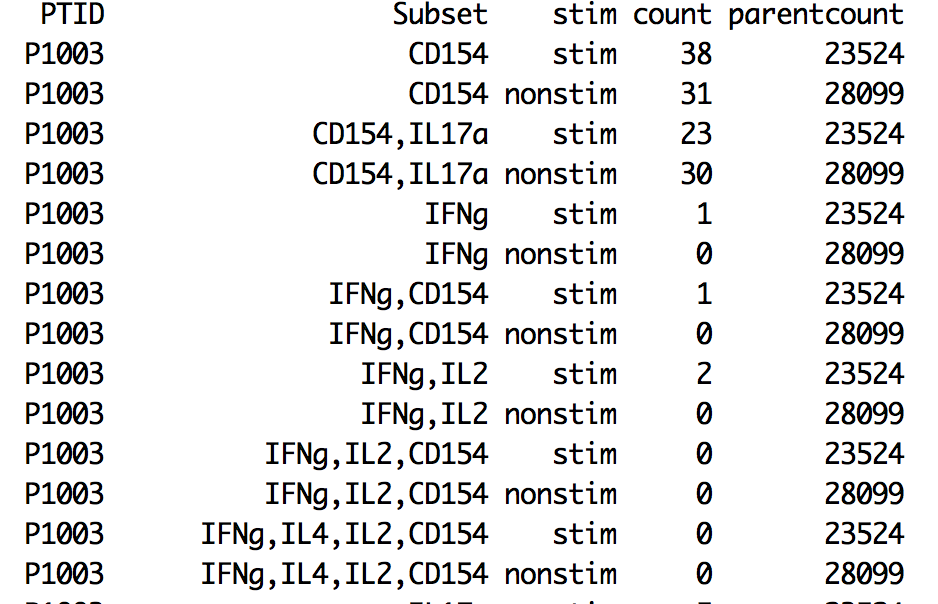
\includegraphics[width=12 cm]{figures/datasetExample} \caption{}
\end{figure}
\end{frame}

%%%%%%%%%%%%%%%%%%%%%%%%%%%%%%%%%%%%%%%%%%%%%%%

\begin{frame}
\frametitle{Analysis Goals} 
\begin{center}
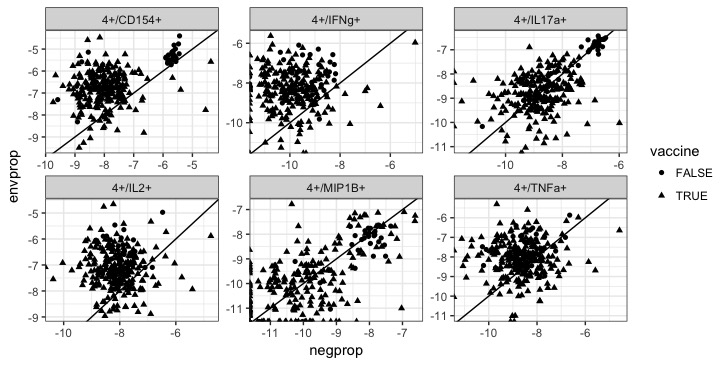
\includegraphics[scale=0.35]{figures/marginalScatterNoPost}
\end{center}
\begin{itemize}
\item Identify cell-subset that exhibit \textbf{vaccine specific response}
\item Identify correlates for succesful \textbf{immunization}
\item Infer \textbf{dependence} structures
\end{itemize}
\end{frame}

%%%%%%%%%%%%%%%%%%%%%%%%%%%%%%%%%%%%%%%%%%%%%%%]

\begin{frame} 
\frametitle{Why a Regression Framework?}

Current solutions are all based on comparing a single control sample to a stimulated sample.
\vspace{0.5 cm}

\begin{itemize}
\item \textbf{Beyond baseline/stimulation}
	\begin{itemize}
	\item Longitudinal data
	\item Multiple stimulations per subject
	\end{itemize}
\vspace{0.65 cm}
	
\item \textbf{Covariates}
	\begin{itemize}
	\item Batch effects
	\item Demographic/background information
	\end{itemize}
\vspace{0.65 cm}

	
\item \textbf{Explicit Dependence Model}
\end{itemize}
\end{frame}

%%%%%%%%%%%%%%%%%%%%%%%%%%%%%%%%%%%%%%%%%%%%%%%]

\begin{frame}
\frametitle{Challenges} 
\begin{center}
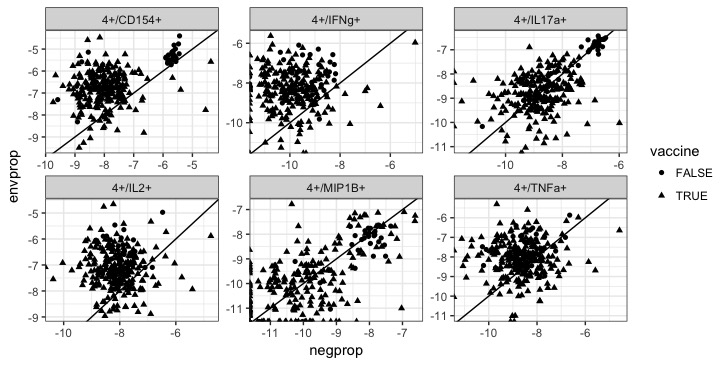
\includegraphics[scale=0.35]{figures/marginalScatterNoPost}
\end{center}
\begin{itemize}
\item \textbf{Overdispersion} (compared to Binomial)
\item Subject specific \textbf{baseline response}
\item Different \textbf{response} patterns
\item \textbf{Dependence} across sub-samples AND cell-subsets
\item \textbf{Dimensionality:} 100+ cell-subsets. 
\end{itemize}
\end{frame}

%%%%%%%%%%%%%%%%%%%%%%%%%%%%%%%%%%%%%%%%%%%%%%%]

\begin{frame}
\frametitle{A Regression Model}
\begin{framed}
Indexing: \textbf{i}-subject, \textbf{t}- subsample, \textbf{j}- subset.
\end{framed}
\begin{itemize}
\item Over-dispersion $\Rightarrow$ \textbf{Beta-Binomial} model: 
$$
\text{logit}(\mu_{ijt}) = X_{ijt}\beta + T_{ijt} z_{ij} + \nu_{ij}
$$$$
y_{ijt} \sim \text{Beta-Binom}(N_{it}, \mu_{ijt}, M_{j})
$$

\vspace{0.5 cm}
\item $X$- Covariates, $\beta$- Regression Coefficients, $T$- Treatment Effects.

\vspace{0.5 cm}
\item Baseline response $\Rightarrow$ $\nu_i \sim N(0, \Sigma)$ 

\vspace{0.5 cm}
\item Differential response $\Rightarrow$ $z_i \in \{0,1\}^{J} \sim Ising(\theta)$.  

\pause
\vspace{0.5 cm}
\item Estimation via a Stochastic-EM algorithm.   
\end{itemize}
\end{frame}

%%%%%%%%%%%%%%%%%%%%%%%%%%%%%%%%%%%%%%%%%%%%%%%

\begin{frame}
\frametitle{The RV144 HIV Vaccine Trial}
\begin{itemize}
\item \textbf{262 Subjects}
	\begin{itemize}
	\item 226 Cases
	\item 36 Controls
	\end{itemize}
\vspace{0.5 cm}

\item \textbf{2 Types of stimulus} 
	\begin{itemize}
	\item HIV protein
	\item Negative control
	\end{itemize}
\vspace{0.5 cm}

\item \textbf{Demographic Information}
	\begin{itemize}
	\item Age
	\item Gender 
	\end{itemize}
\vspace{0.5 cm}

\item \textbf{23 CD4 Cell-Subsets.} 
\end{itemize}
\end{frame}

%%%%%%%%%%%%%%%%%%%%%%%%%%%%%%%%%%%%%%%%%%%%%%%

\begin{frame}
\frametitle{The Plan}
\begin{enumerate}
\item Fit the model based on \textbf{count data}:
$$
\text{logit}(\mu_{ijt}) = \beta_0 + \beta_1\text{age}_i + \beta_2\text{gender}_i + z_{ij}\tau_{j}\text{stimulation}_{ijt} + \nu_{ij}
$$

\textbf{Outputs:}
	\begin{itemize}
	\item Regression coefficient estimates
	\item Posterior response probabilities
	\item Covariance for random effects
	\item Estimated graphical model
	\end{itemize}

\pause
\vspace{0.5 cm}
\item Validate inferred quantities using \textbf{vaccination} data.
 
 \vspace{0.5 cm}
\item Formulate hypothesis and test using \textbf{infection} data. 
\end{enumerate}
\end{frame}

%%%%%%%%%%%%%%%%%%%%%%%%%%%%%%%%%%%%%%%%%%%%%%%

\begin{frame}
\frametitle{RV144 - Booleans Dataset}
\begin{figure}[]
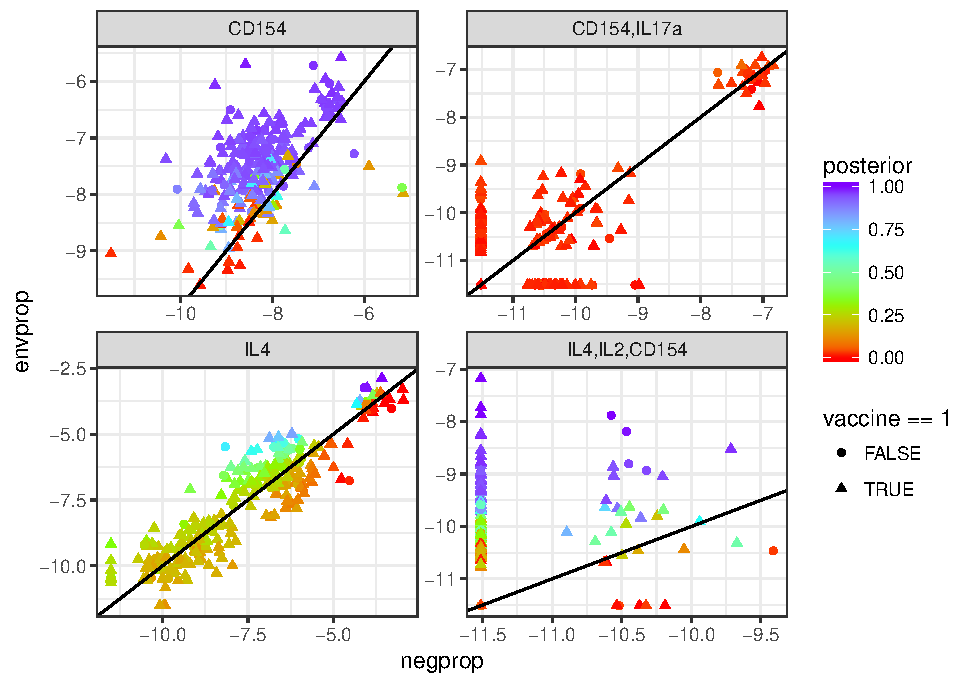
\includegraphics[width=\maxwidth]{figures/updatedRV144scatter} 
\end{figure}
\end{frame}

%%%%%%%%%%%%%%%%%%%%%%%%%%%%%%%%%%%%%%%%%%%%%%%]

\begin{frame}
\frametitle{RV144 - Booleans Dataset}
\begin{figure}[]
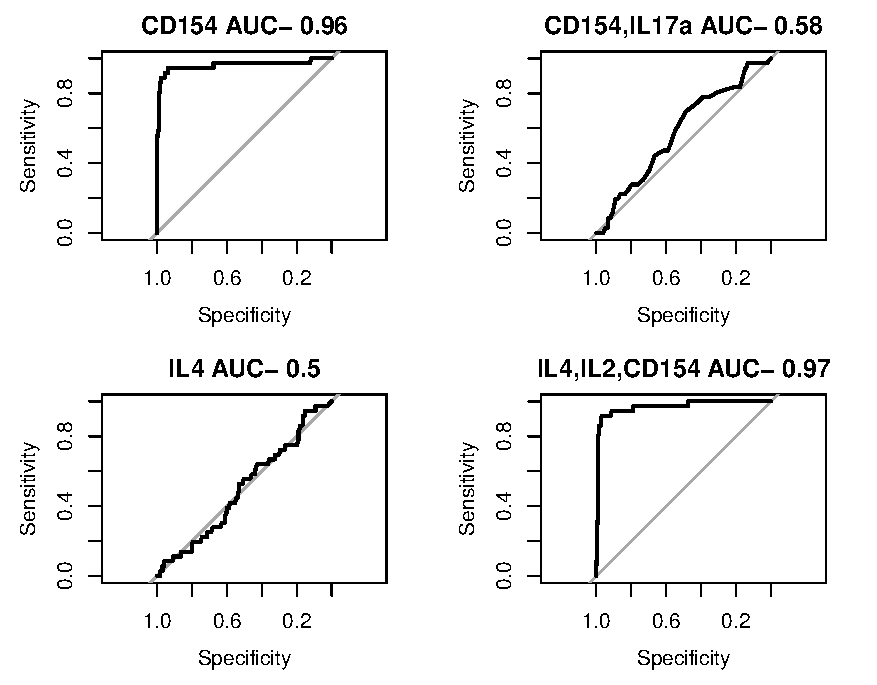
\includegraphics[width=\maxwidth]{figures/RV144newROCsmall}
\end{figure}
\end{frame}

%%%%%%%%%%%%%%%%%%%%%%%%%%%%%%%%%%%%%%%%%%%%%%%]

\begin{frame}
\frametitle{An Informative Graphical Model}
\begin{figure}[]
\includegraphics[width= \maxwidth]{figures/rv144newNetworkAuc} 
\end{figure}
\end{frame}

%%%%%%%%%%%%%%%%%%%%%%%%%%%%%%%%%%%%%%%%%%%%%%%]

\begin{frame}
\frametitle{ROC for Vaccination/Placebo}
\begin{figure}[]
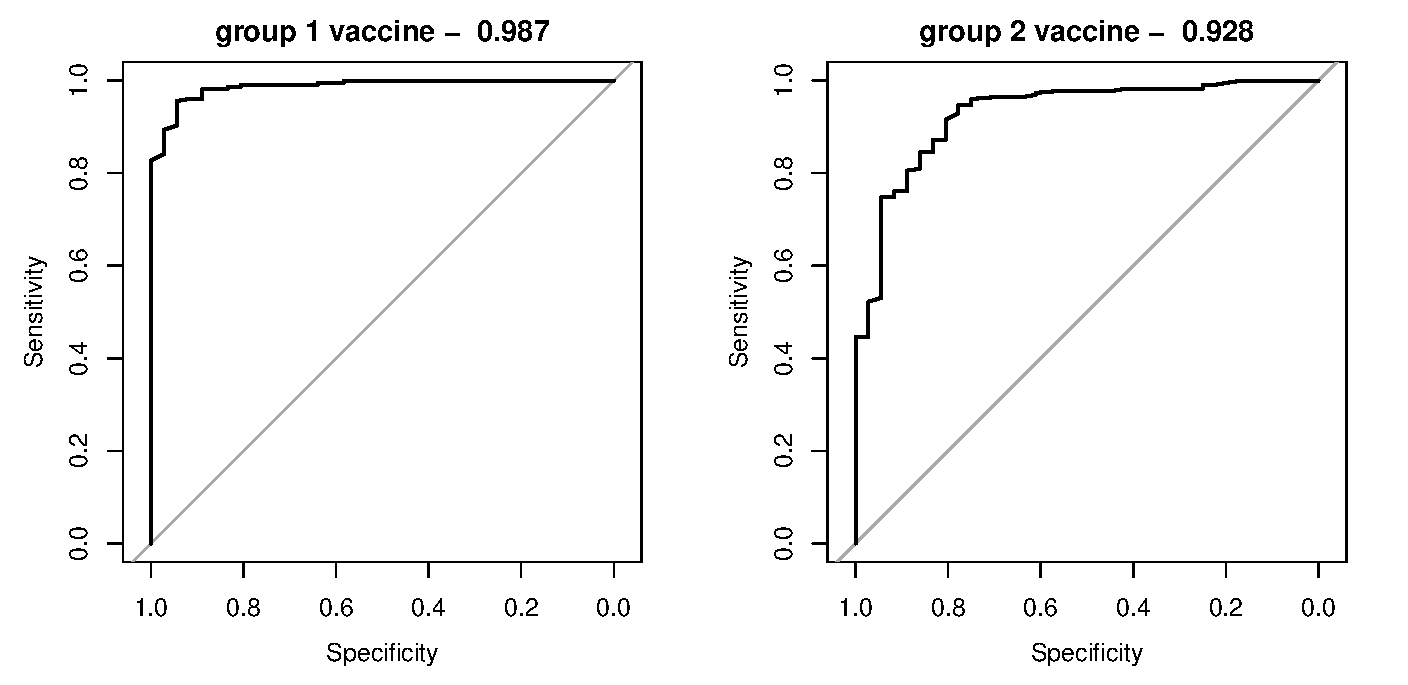
\includegraphics[width= \maxwidth]{figures/rv144ComponentROCvaccine} 
\end{figure}
$$
\text{ROC}(\text{vaccine} \sim s_j), \qquad s_{ij} = \frac{1}{|C_j|}\sum_{i \in C_j} \text{post}_{ij}
$$
\end{frame}

%%%%%%%%%%%%%%%%%%%%%%%%%%%%%%%%%%%%%%%%%%%%%%%]

\begin{frame}
\frametitle{ROC for Infection Status} 
\begin{figure}[]
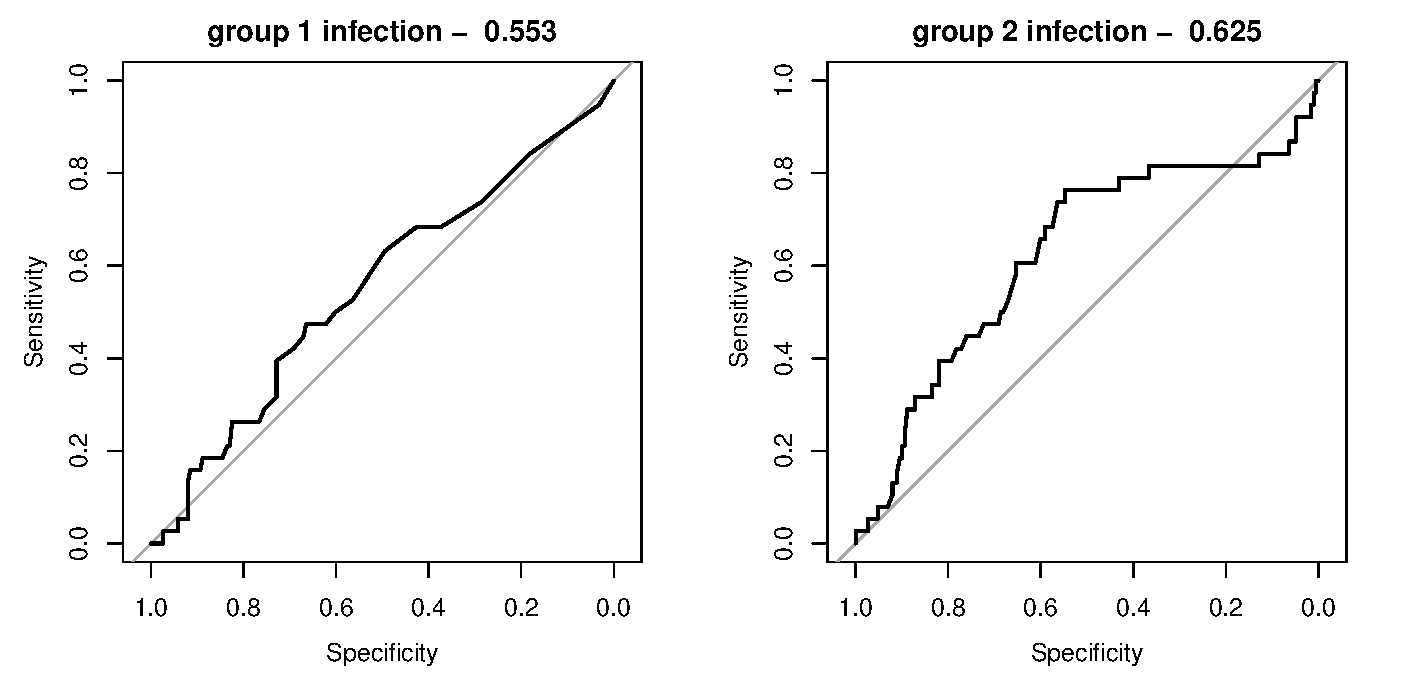
\includegraphics[width= \maxwidth]{figures/RV144componentInfection} 
\end{figure}

\textbf{AUC of $\boldsymbol{0.625}$ $\boldsymbol{\Rightarrow}$ p-value of $\boldsymbol{0.007}$.}
\end{frame}

%%%%%%%%%%%%%%%%%%%%%%%%%%%%%%%%%%%%%%%%%%%%%%%]

\begin{frame}
\frametitle{The HVTN 505 Vaccine Trial}
\begin{itemize}
\item \textbf{238 Subjects}
	\begin{itemize}
	\item 189 Cases
	\item 49 Controls
	\end{itemize}
\vspace{0.4 cm}
\item \textbf{5 Types of stimulus} 
	\begin{itemize}
	\item 4 types of HIV proteins (ENV, GAG, POL, NEF).
	\item Negative control.
	\item Multiple samples per stimulation.
	\end{itemize}
\vspace{0.4 cm}
\item \textbf{52 Cell Subsets}
	\begin{itemize}
	\item $25$ CD4 cells.
	\item $27$ CD8 cells.
	\end{itemize} 
\end{itemize}
\end{frame}

%%%%%%%%%%%%%%%%%%%%%%%%%%%%%%%%%%%%%%%%%%%%%%%]

\begin{frame}
\frametitle{Inferred Graph for HVTN505}
\begin{figure}[]
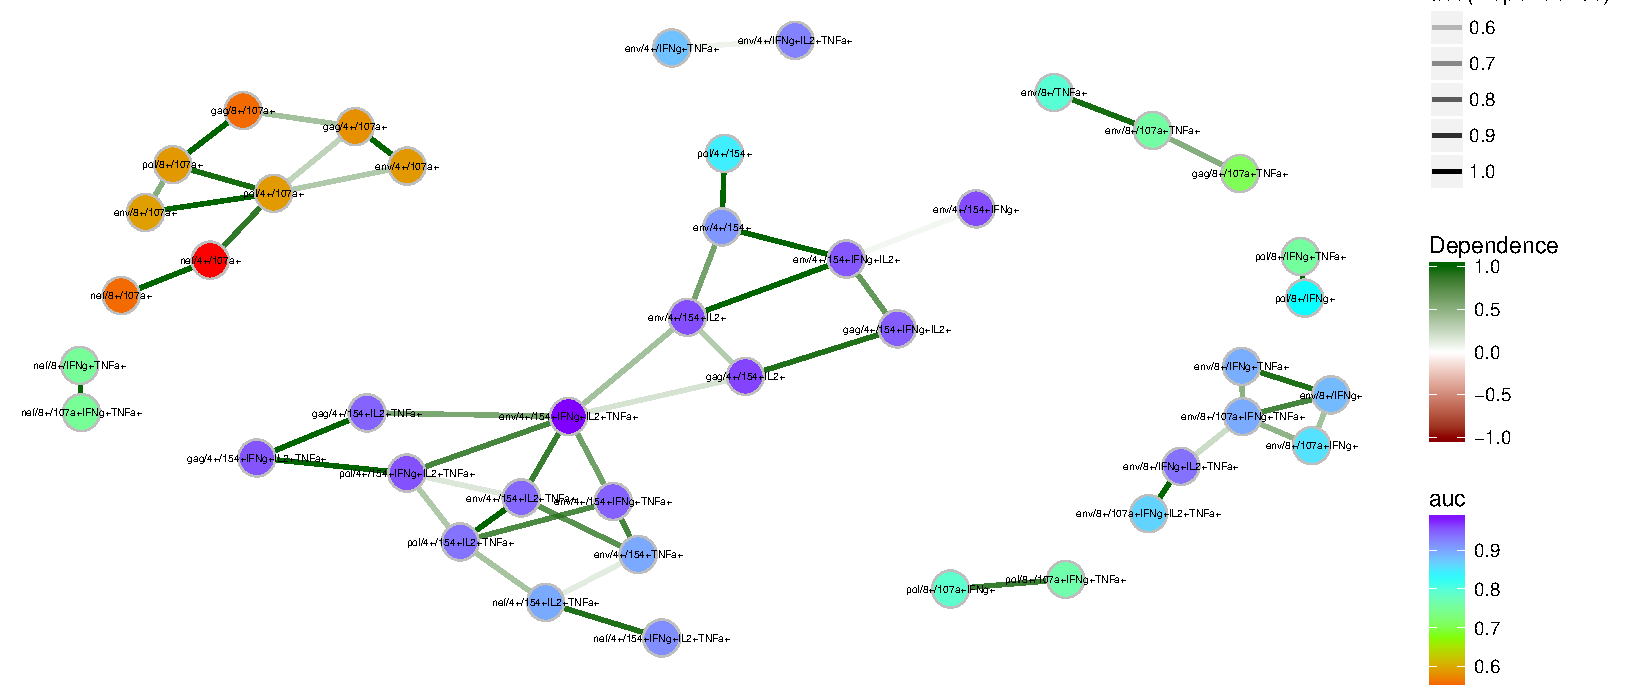
\includegraphics[width=\maxwidth]{figures/HVTNrobustNetwork}
\end{figure}
\end{frame}

%%%%%%%%%%%%%%%%%%%%%%%%%%%%%%%%%%%%%%%%%%%%%%%]

\begin{frame}
\frametitle{Color Coded by AUCs for Vaccination/Placebo}
\begin{figure}[]
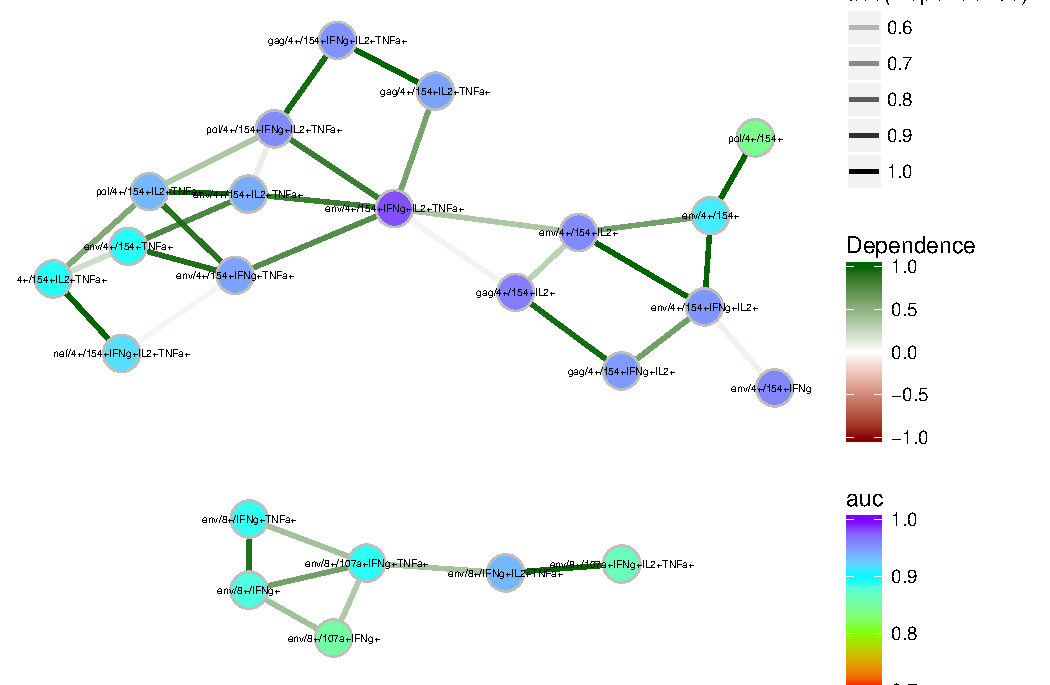
\includegraphics[width=\maxwidth]{figures/twoComponentVaccine}
\end{figure}
\end{frame}

%%%%%%%%%%%%%%%%%%%%%%%%%%%%%%%%%%%%%%%%%%%%%%%]

\begin{frame}
\frametitle{Color Coded by AUCs for Infection Status}
\begin{figure}[]
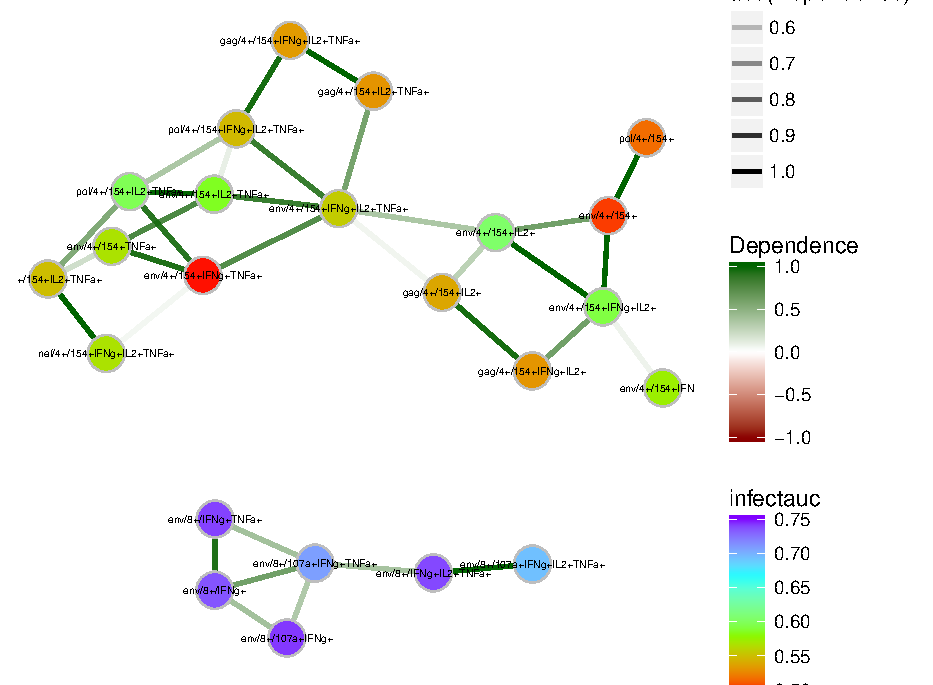
\includegraphics[width=\maxwidth]{figures/twoComponentInfect}
\end{figure}
\end{frame}

%%%%%%%%%%%%%%%%%%%%%%%%%%%%%%%%%%%%%%%%%%%%%%%]



\begin{frame}
\frametitle{ROC for Vaccination/Placebo}
\begin{figure}[]
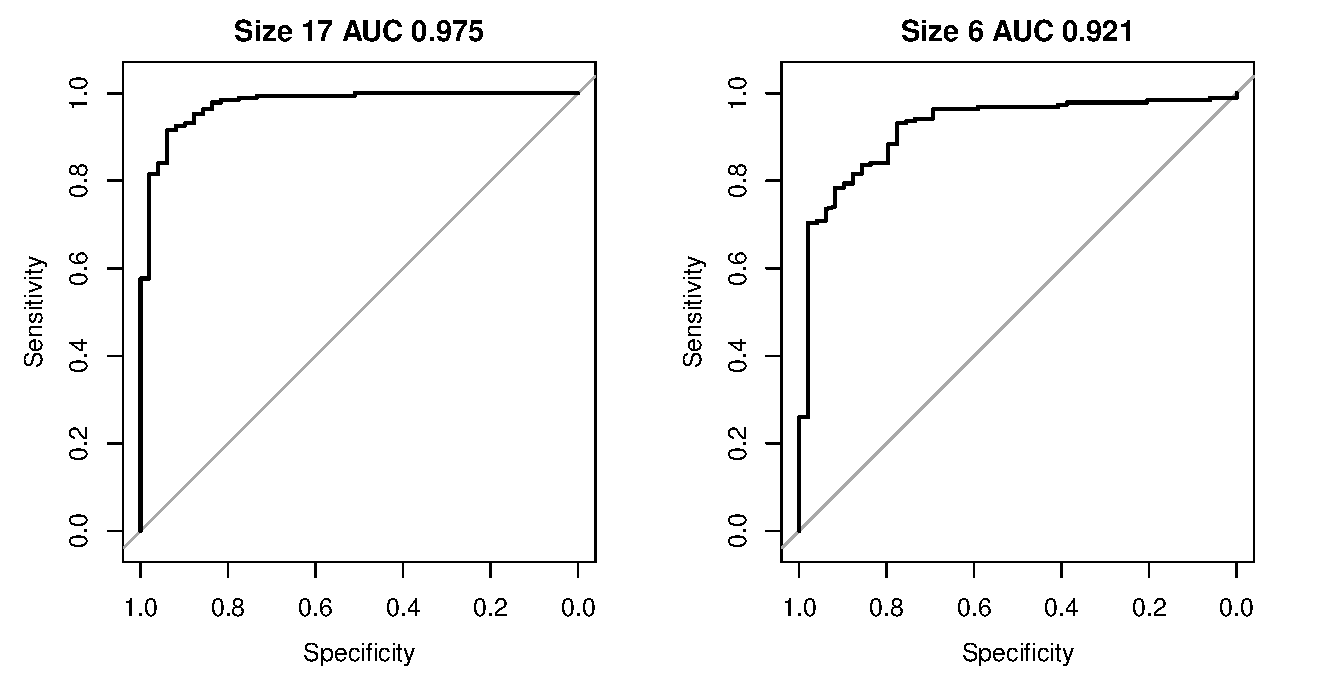
\includegraphics[width= \maxwidth]{figures/HVTNcompROCvacc} 
\end{figure}
\end{frame}

%%%%%%%%%%%%%%%%%%%%%%%%%%%%%%%%%%%%%%%%%%%%%%%]

\begin{frame}
\frametitle{ROC for Infection Status} 
\begin{figure}[]
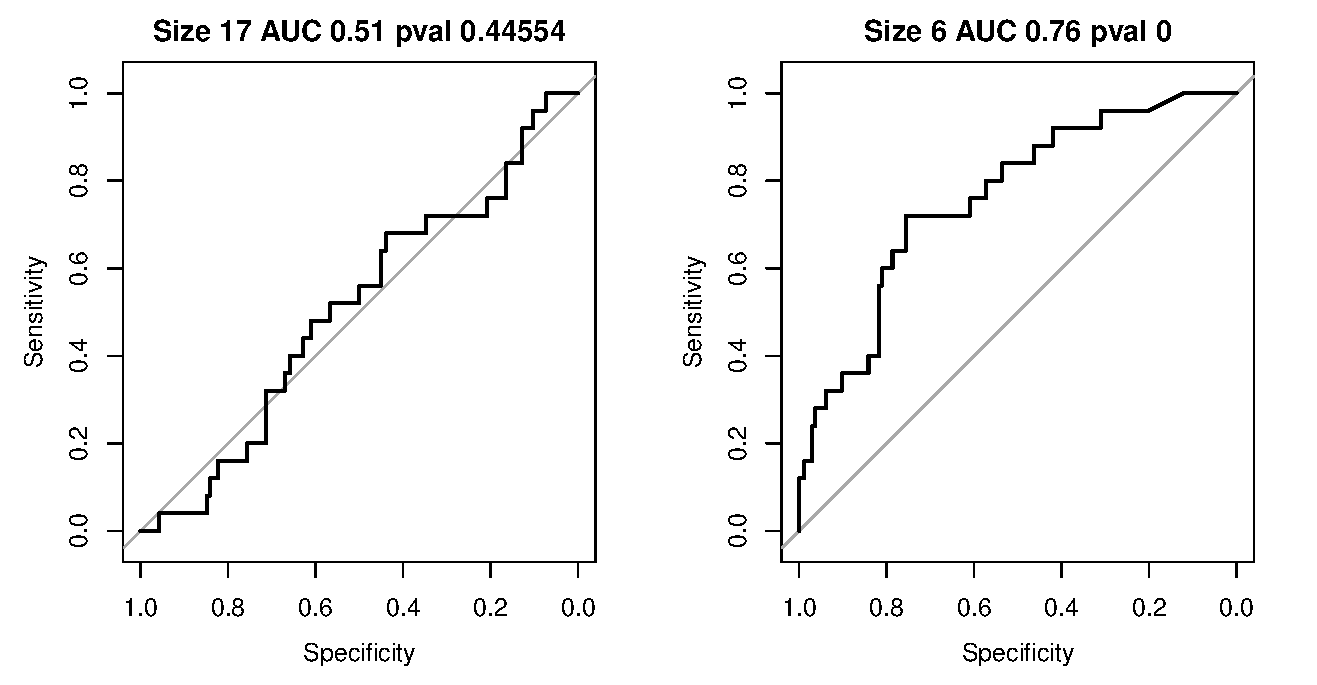
\includegraphics[width= \maxwidth]{figures/HVTNcompROCinfect} 
\end{figure}

\textbf{AUC of $\boldsymbol{0.76}$ $\boldsymbol{\Rightarrow}$ p-value of $\boldsymbol{ \approx 10^{-8}}$.}
\end{frame}

%%%%%%%%%%%%%%%%%%%%%%%%%%%%%%%%%%%%%%%%%%%%%%%]

\begin{frame}
\frametitle{Conclusion}
\begin{itemize}
\item We developed a regression model which allows for the analysis of complex cell-count datasets.
	\begin{itemize}
	\item Multiple time-points/observations per subject. 
	\item Batch effects
	\item Demographic Information
	\end{itemize}

\vspace{0.7 cm}
\item  We model the dependence structure explicitly via a sparse graphical model.
	\begin{itemize}
	\item Identified subsets predictive of vaccination \textbf{or} immunization.	
	\end{itemize}
	
\vspace{0.7 cm}
\item  What else?
	\begin{itemize}
	\item Longitudinal data
	\item Enrichment Analysis
	\item Aggregate measures of response
	\end{itemize}
\end{itemize}
\end{frame}

%%%%%%%%%%%%%%%%%%%%%%%%%%%%%%%%%%%%%%%%%%%%%%%]

\begin{frame}
\begin{center}
\huge{Thank you!}

\vspace{2 cm}
\LARGE{Questions?}

\vspace{1cm}
\large{AmitMeir@uw.edu}
\end{center}
\end{frame}

%%%%%%%%%%%%%%%%%%%%%%%%%%%%%%%%%%%%%%%%%%%%%%%]

\begin{frame}
\frametitle{Analysis Goals}
\begin{itemize}
\item \textbf{Problem:} We are interested in identifying response in Subsets X Protein pairs. 

\vspace{0.75 cm}
\item \textbf{Solution:} Treat each combination of Subset X Protein as a cell-subset.
	\begin{itemize}
	\item Overall 120 subsets with non-negligible counts. 
	\end{itemize}

\vspace{0.75 cm}
\item Dependence structures should (and do!) sort themselves out.
\end{itemize}
\end{frame}

%%%%%%%%%%%%%%%%%%%%%%%%%%%%%%%%%%%%%%%%%%%%%%%]

\begin{frame}
\frametitle{RV144 - Booleans Dataset}
\begin{figure}[]
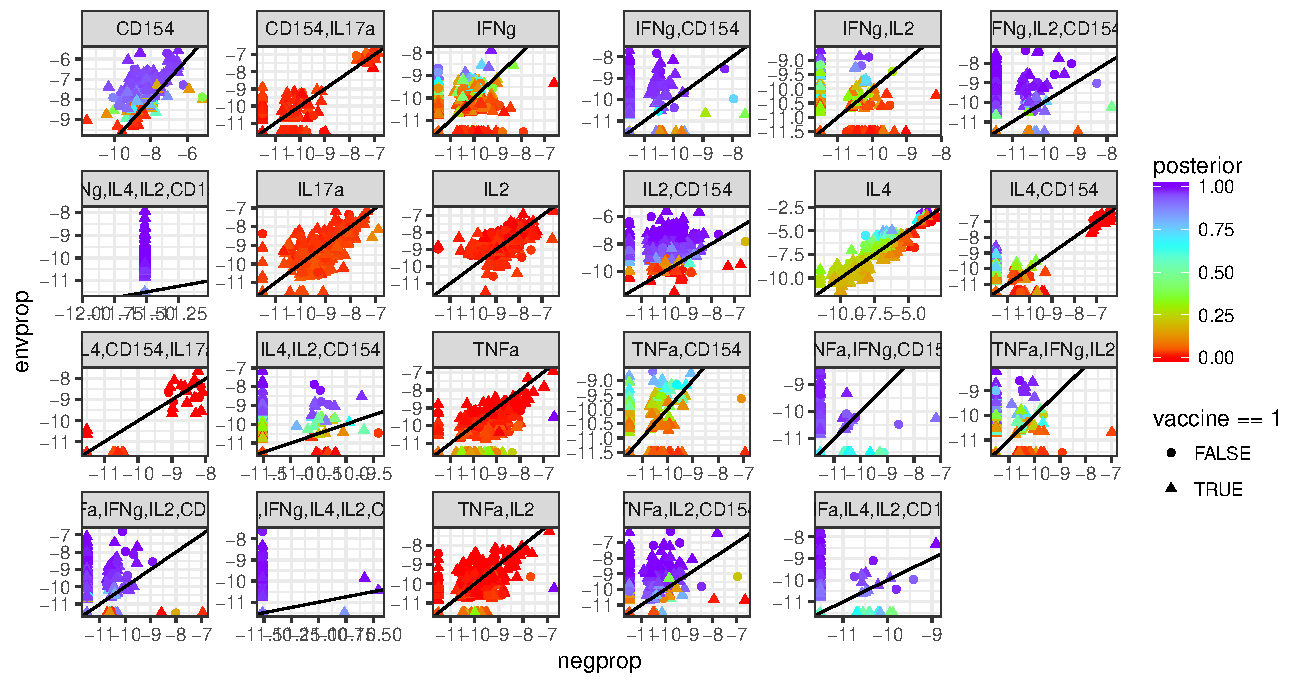
\includegraphics[width=\maxwidth]{figures/newRV144all} 
\end{figure}
\end{frame}

%%%%%%%%%%%%%%%%%%%%%%%%%%%%%%%%%%%%%%%%%%%%%%%]

\end{document}